\chapter{Diseño}
\label{chap:diseño}

\lettrine{P}{ara} abordar el diseño de la aplicación se detallará, a lo largo de este capítulo, la arquitectura software elegida para el sistema,
se mostrarán los prototipos de la interfaz de usuario elaborados y se explicará a fondo mediante diagramas de clases la estructura a bajo nivel
tanto del \textit{frontend} como del \textit{backend}.

\section{Arquitectura}
\label{sec:diseño_arquitectura}

Teniendo en cuenta los requisitos definidos en las Secciones \ref{sec:analisis_requisitos_funcionales} y \ref{sec:analisis_requisitos_no_funcionales},
así como también las limitaciones temporales del proyecto, se ha optado por una arquitectura cliente-servidor. Esta aquitectura se ha elegido
por la facilidad en su implementación y por su capacidad de intercomunicación con otros sistemas, especialmente con clientes web. Como
se aprecia en la Figura \ref{fig:arquitectura_contenedor}, el servidor cuenta con un controlador REST capaz de redirigir las peticiones al servicio
corresepondiente. En este sentido, a pesar de solo contar con un único servicio en la versión actual (\textit{Servicio de perfilado}),
la arquitectura cliente-servidor permite añadir nuevos servicios, junto a nuevas funcionalidades, de forma sencilla y sin poner en riesgo al resto del sistema.
Dicho servicio será el que se comunique con la base da datos para garantizar la persistencia de los datos del perfilado y permitir así
una posterior consulta.

\bigskip
Por otro lado, para que el código estuviese bien organizado, se decidió utilizar el patrón de diseño DDD (del inglés \textit{Domain-Driven Design}) \cite{ddd}, el cual
permite separar el código en tres capas: la capa de aplicación, la capa de dominio y la capa de infraestructura. La capa de aplicación es la encargada de gestionar
la entrada y salida de la aplicación que, en nuestro caso, es el controlador que maneja los \textit{endpoints} REST; la capa de dominio es la que contiene la lógica
de negocio y las entidades; y la capa de infraestructura es la responsable de administrar las interacciones internas de la aplicación que, en nuestro
caso, se encarga de la comunicación con la base de datos.

\begin{figure}[H]
	\centering
	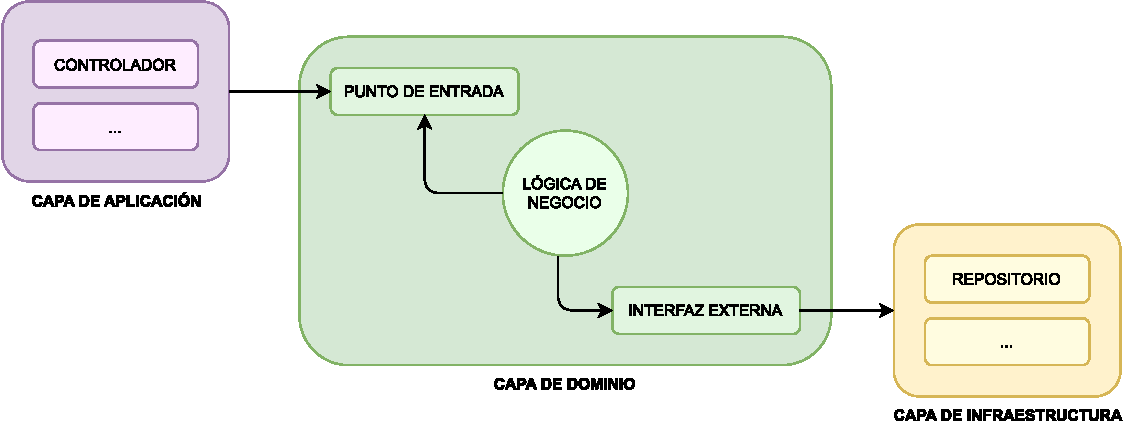
\includegraphics[width=0.9\textwidth]{diagramas/ddd.pdf}
	\caption{Diagrama de capas del patrón de diseño DDD. Adaptado de Ł, Ryś \cite{dddblog}}
	\label{fig:ddd}
\end{figure}

\bigskip
A mayores, el propio \textit{frontend} web tendrá también una arquitectura basada en cliente-servidor, en la que el servidor será el encargado
de ofrecer al cliente los archivos estáticos necesarios para mostrar la interfaz (HTML, CSS, JavaScript, fuentes, imágenes...). El hecho
de elegir una interfaz web gira en torno al requisito no funcional de portabilidad (\hyperref[req:rnf3]{RNF3}),
puesto que, de esta forma, la aplicación podría ser utilizada por cualquier dispositivo con un navegador, evitando
desarrollar aplicaciones nativas para cada sistema operativo.

\bigskip
\begin{figure}[H]
	\centering
	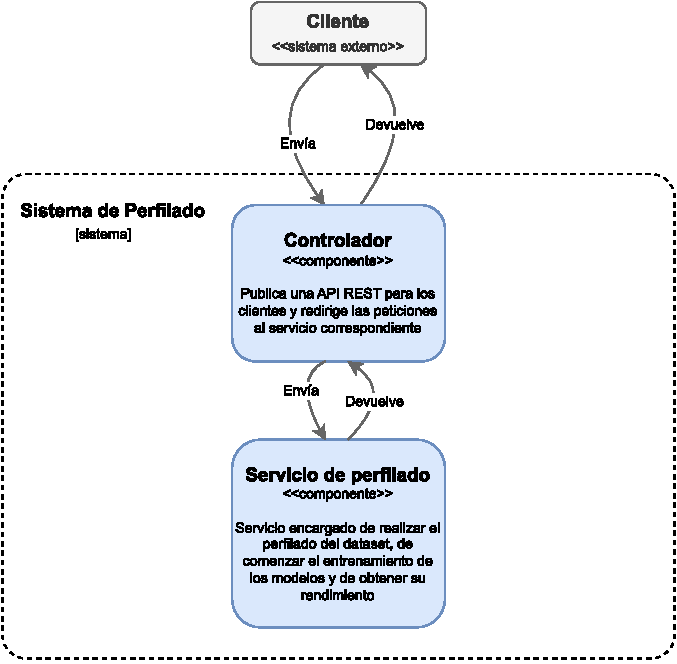
\includegraphics[width=0.7\textwidth]{diagramas/arquitectura_contenedor.pdf}
	\caption{Diagrama C4 de Contenedor de la arquitectura del sistema.}
	\label{fig:arquitectura_contenedor}
\end{figure}

\section{Prototipado}
\label{sec:diseño_prototipado}

Como se mencionó anteriormente, para el diseño de los prototipos de pantallas, también conocidos como \textit{wireframes}, se utilizó
la herramienta Draw.io \cite{drawio} debido a su sencillez y rapidez en la elaboración con respecto a otros programas más avanzados
como pueden ser Adobe XD \cite{adobexd} o Figma \cite{figma}.

\bigskip
La filosofía de diseño de la interfaz se centró en el minimalismo y la accesibilidad, como se establece en el \hyperref[req:rnf1]{RNF1}
recogido en la Sección \ref{sec:analisis_requisitos_no_funcionales}, por lo que todo está caracterizado por no contener excesivos elementos y por ser fácilmente comprensible para el usuario.

\bigskip
La pantalla de inicio, como se ve en la Figura \ref{fig:prototipo_inicio}, está compuesta simplemente por un título,
un subtítulo y un campo que dará la opción al usuario de subir un \textit{dataset}, tanto mediante un elemento \textit{drag and drop} como
mediante un botón que permitirá la selección de un archivo almacenado en el dispositivo.

\bigskip
\begin{figure}[H]
	\centering
	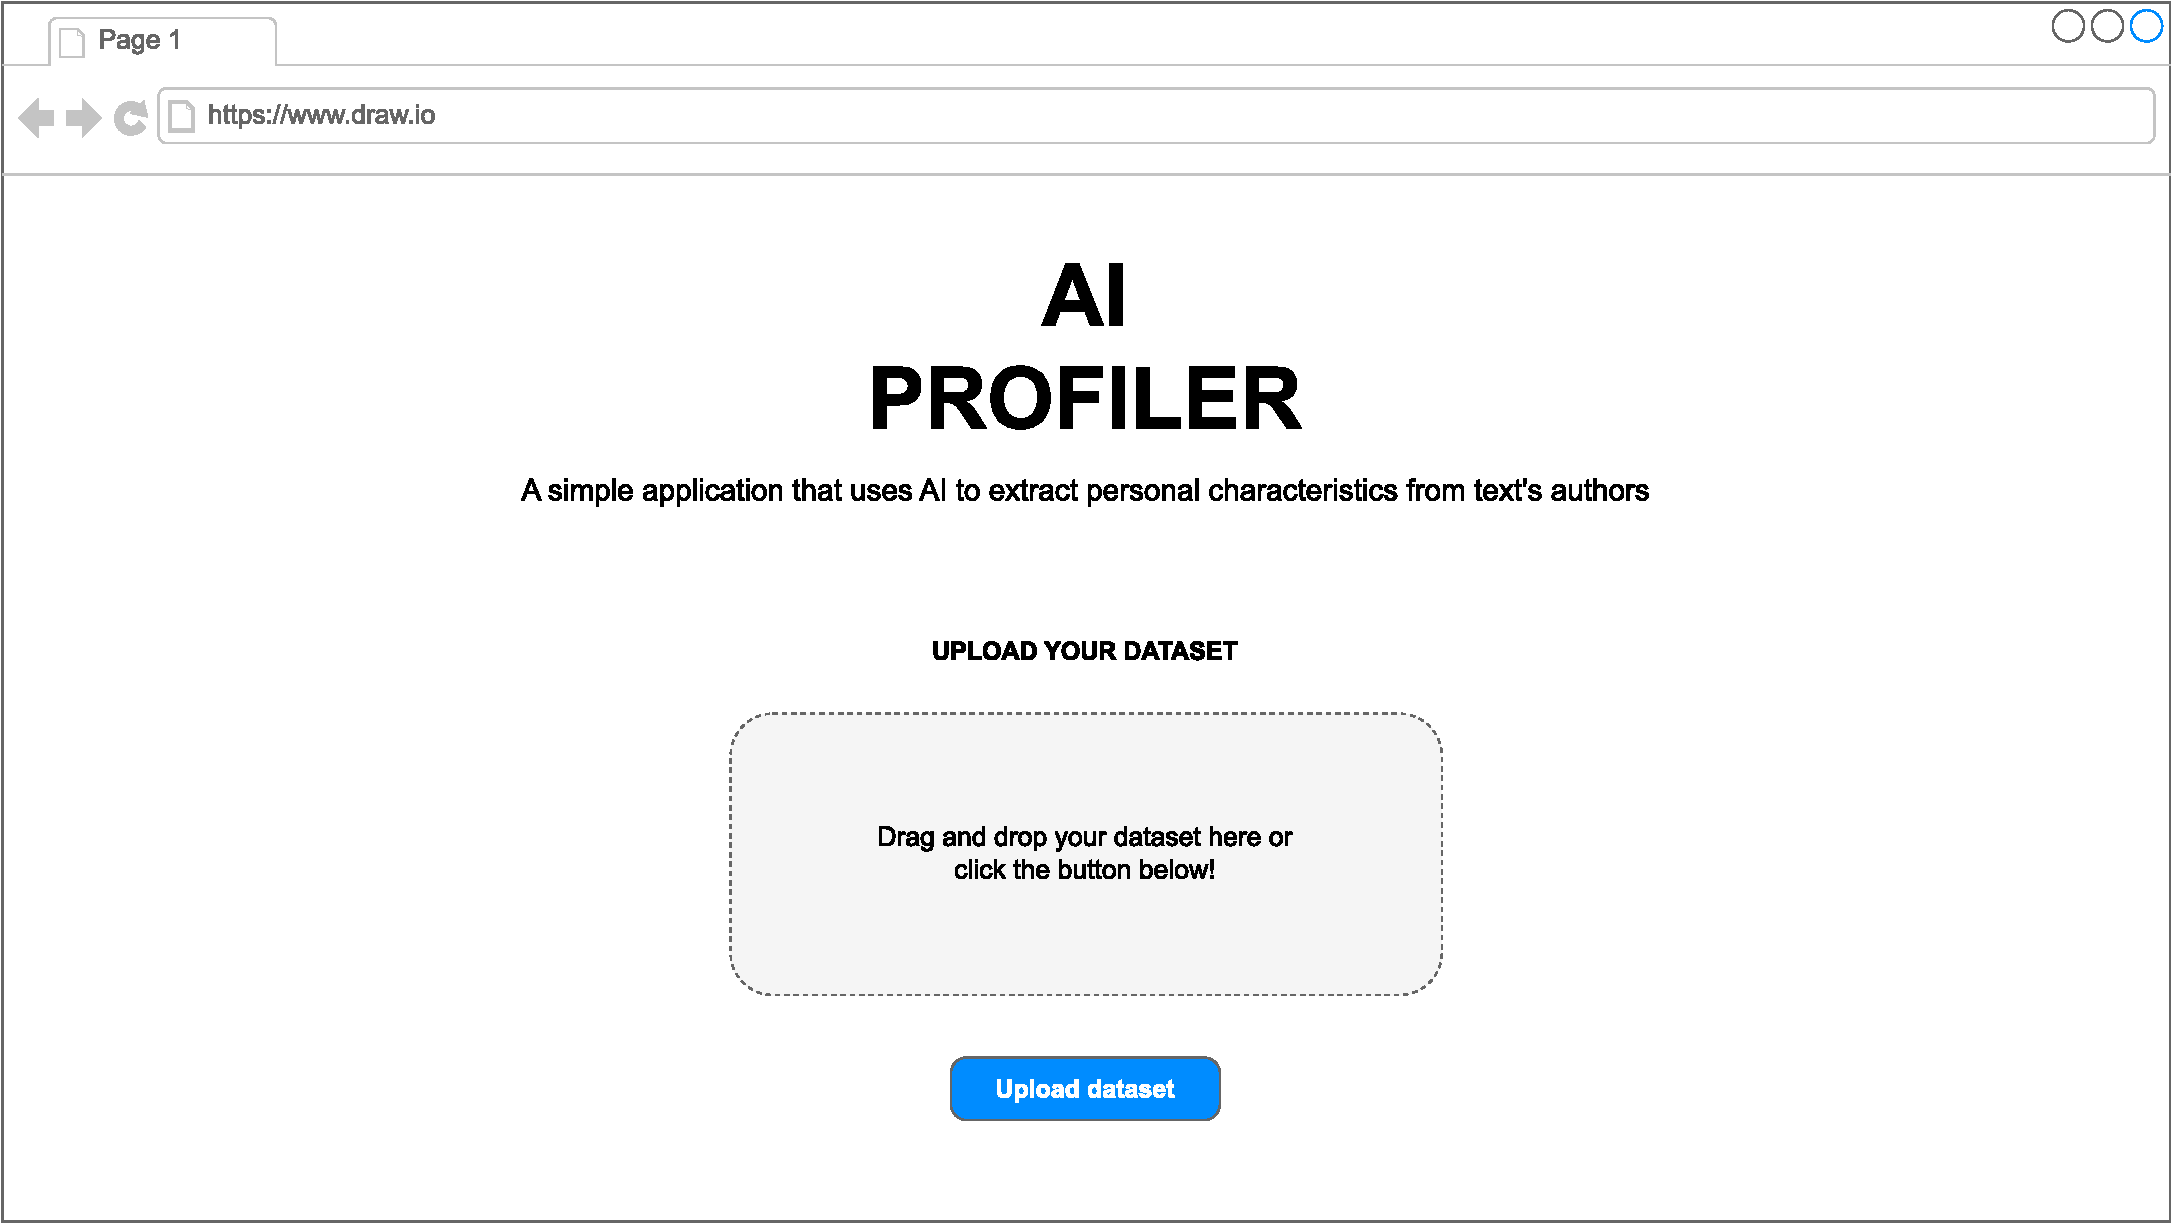
\includegraphics[width=\textwidth]{diagramas/landing.pdf}
	\caption{Prototipo de la pantalla de inicio}
	\label{fig:prototipo_inicio}
\end{figure}

\bigskip
Una vez el usuario haya subido el \textit{dataset}, el campo de subida se sustituirá por la lista de los
algoritmos de perfilado disponibles, como se puede ver en la Figura \ref{fig:prototipo_algoritmo_perfilado}. De cada algoritmo se mostrará,
en una tarjeta, su nombre junto a las características demográficas que es capaz de extraer. Además, ya que según indican las historias de usuario \hyperref[req:hu7]{H7} y \hyperref[req:hu8]{H8},
era necesario mostrar información del funcionamiento
y del rendimiento de los algoritmos, se decidió crear un mensaje emergente (\textit{tooltip} en inglés) para ello. Un \textit{tooltip} es una ventana
que aparece al pasar el ratón por encima de un elemento y que muestra información adicional sobre el mismo sin ocupar espacio
en la interfaz. Finalmente, si el usuario desease cambiar el \textit{dataset} seleccionado, se permitirá retroceder mediante
la flecha situada junto al título del paso actual.

\bigskip
\begin{figure}[H]
	\centering
	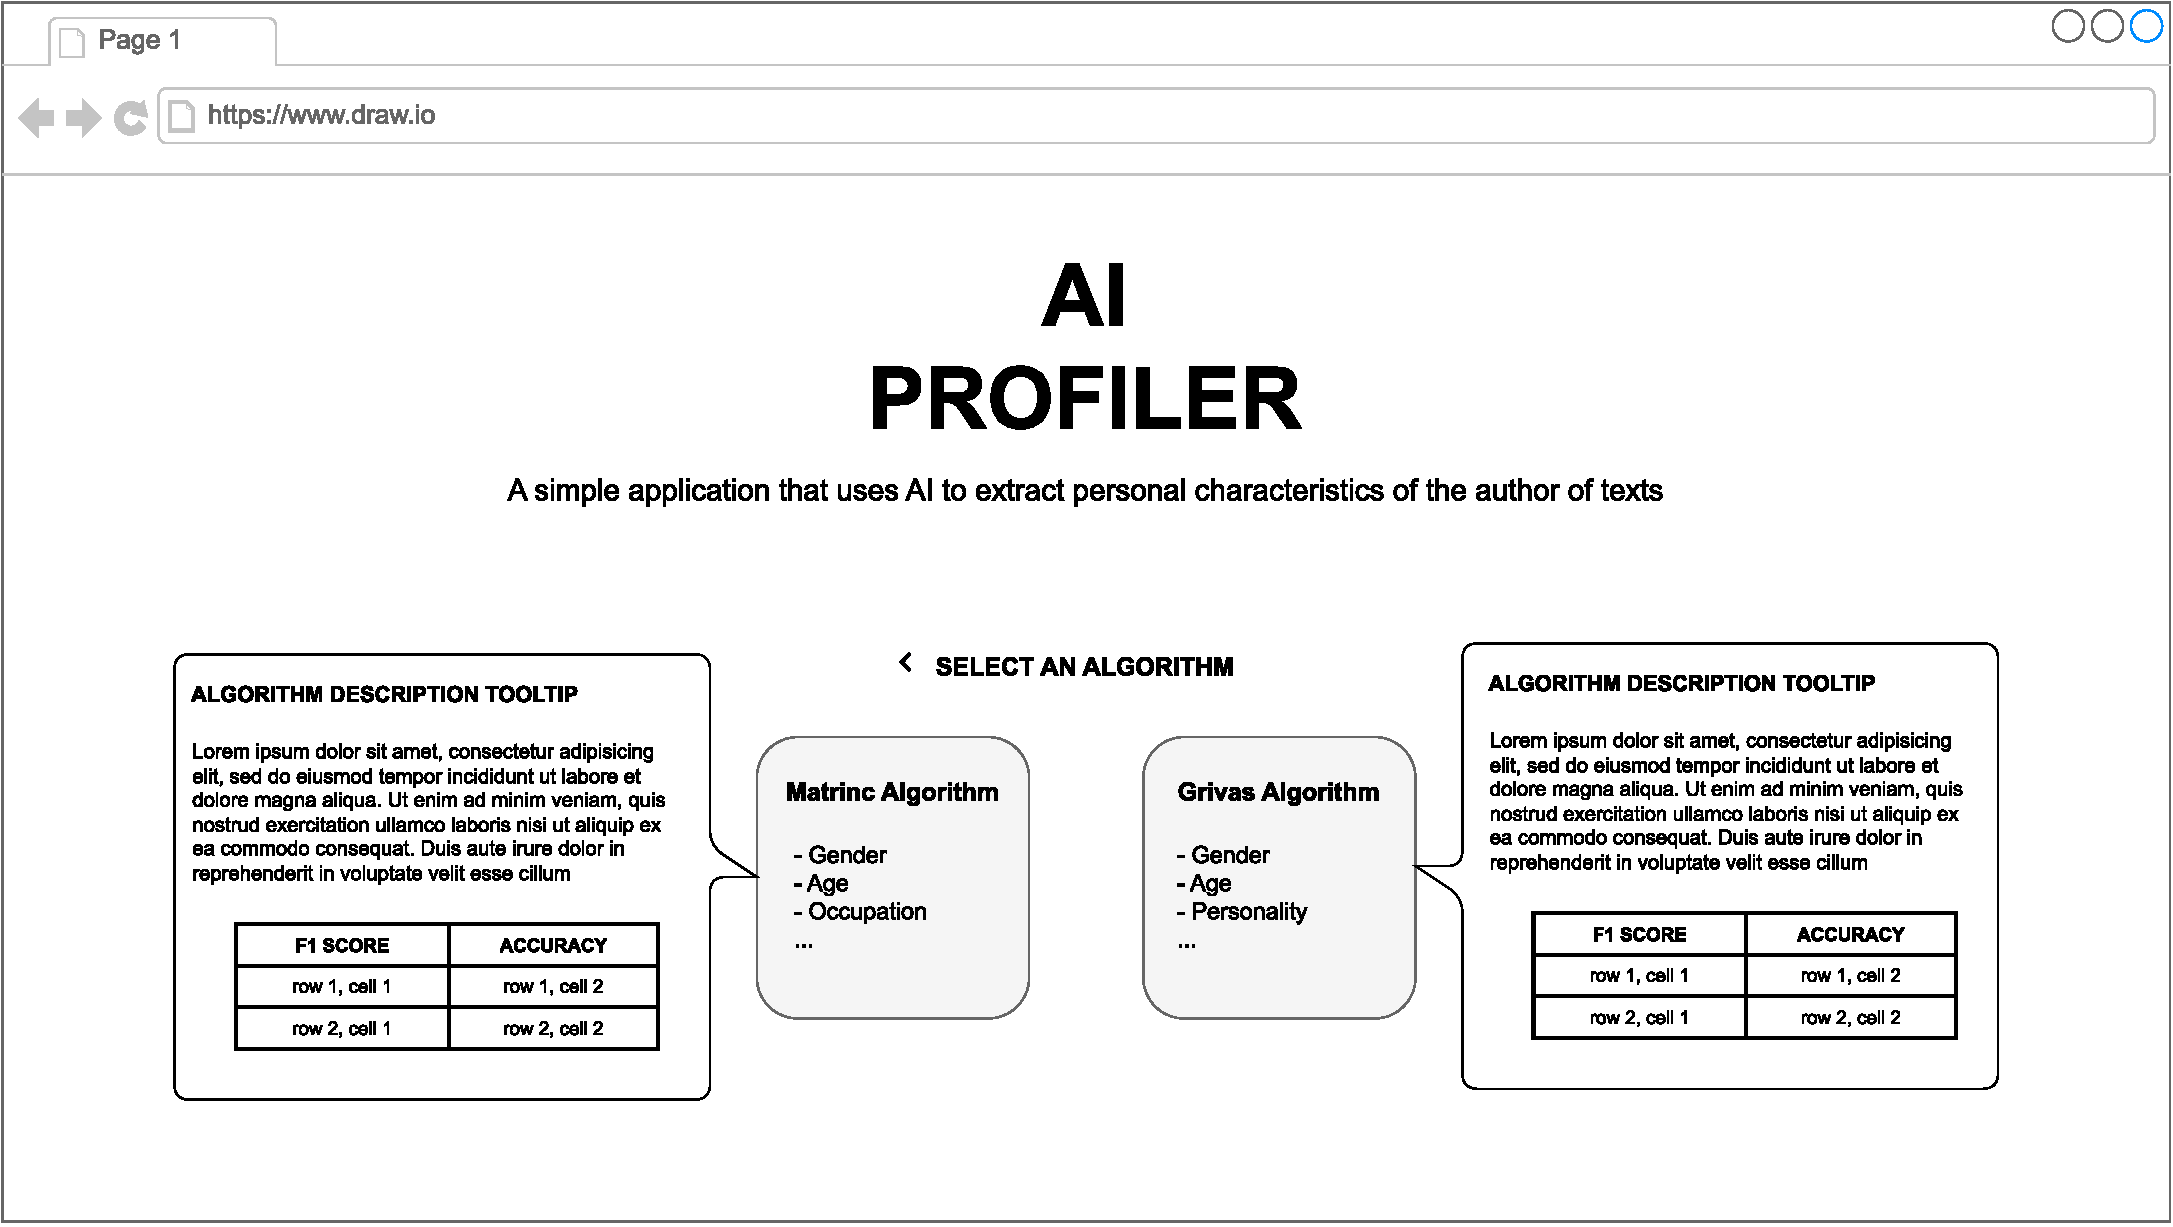
\includegraphics[width=\textwidth]{diagramas/landing-algorithm.pdf}
	\caption{Prototipo de la selección del algoritmo de perfilado}
	\label{fig:prototipo_algoritmo_perfilado}
\end{figure}

\bigskip
Ya con el \textit{dataset} y el algoritmo seleccionados, se presentará al usuario un resumen del perfilado, donde se mostrará
el nombre del fichero subido, la tarjeta del algoritmo seleccionado y un botón que permitirá comenzar con el proceso.
Además, como se aprecia en la Figura \ref{fig:prototipo_resumen_perfilado}, una vez comienza el perfilado, se mostrará una barra de progreso
o un \textit{spinner} que le indicará al usuario que el proceso está en marcha. De la misma forma que en el paso anterior, si el usuario
decide cambiar de algoritmo, puede retroceder haciendo uso de la flecha situada junto al título del paso actual.

\bigskip
\begin{figure}[H]
	\centering
	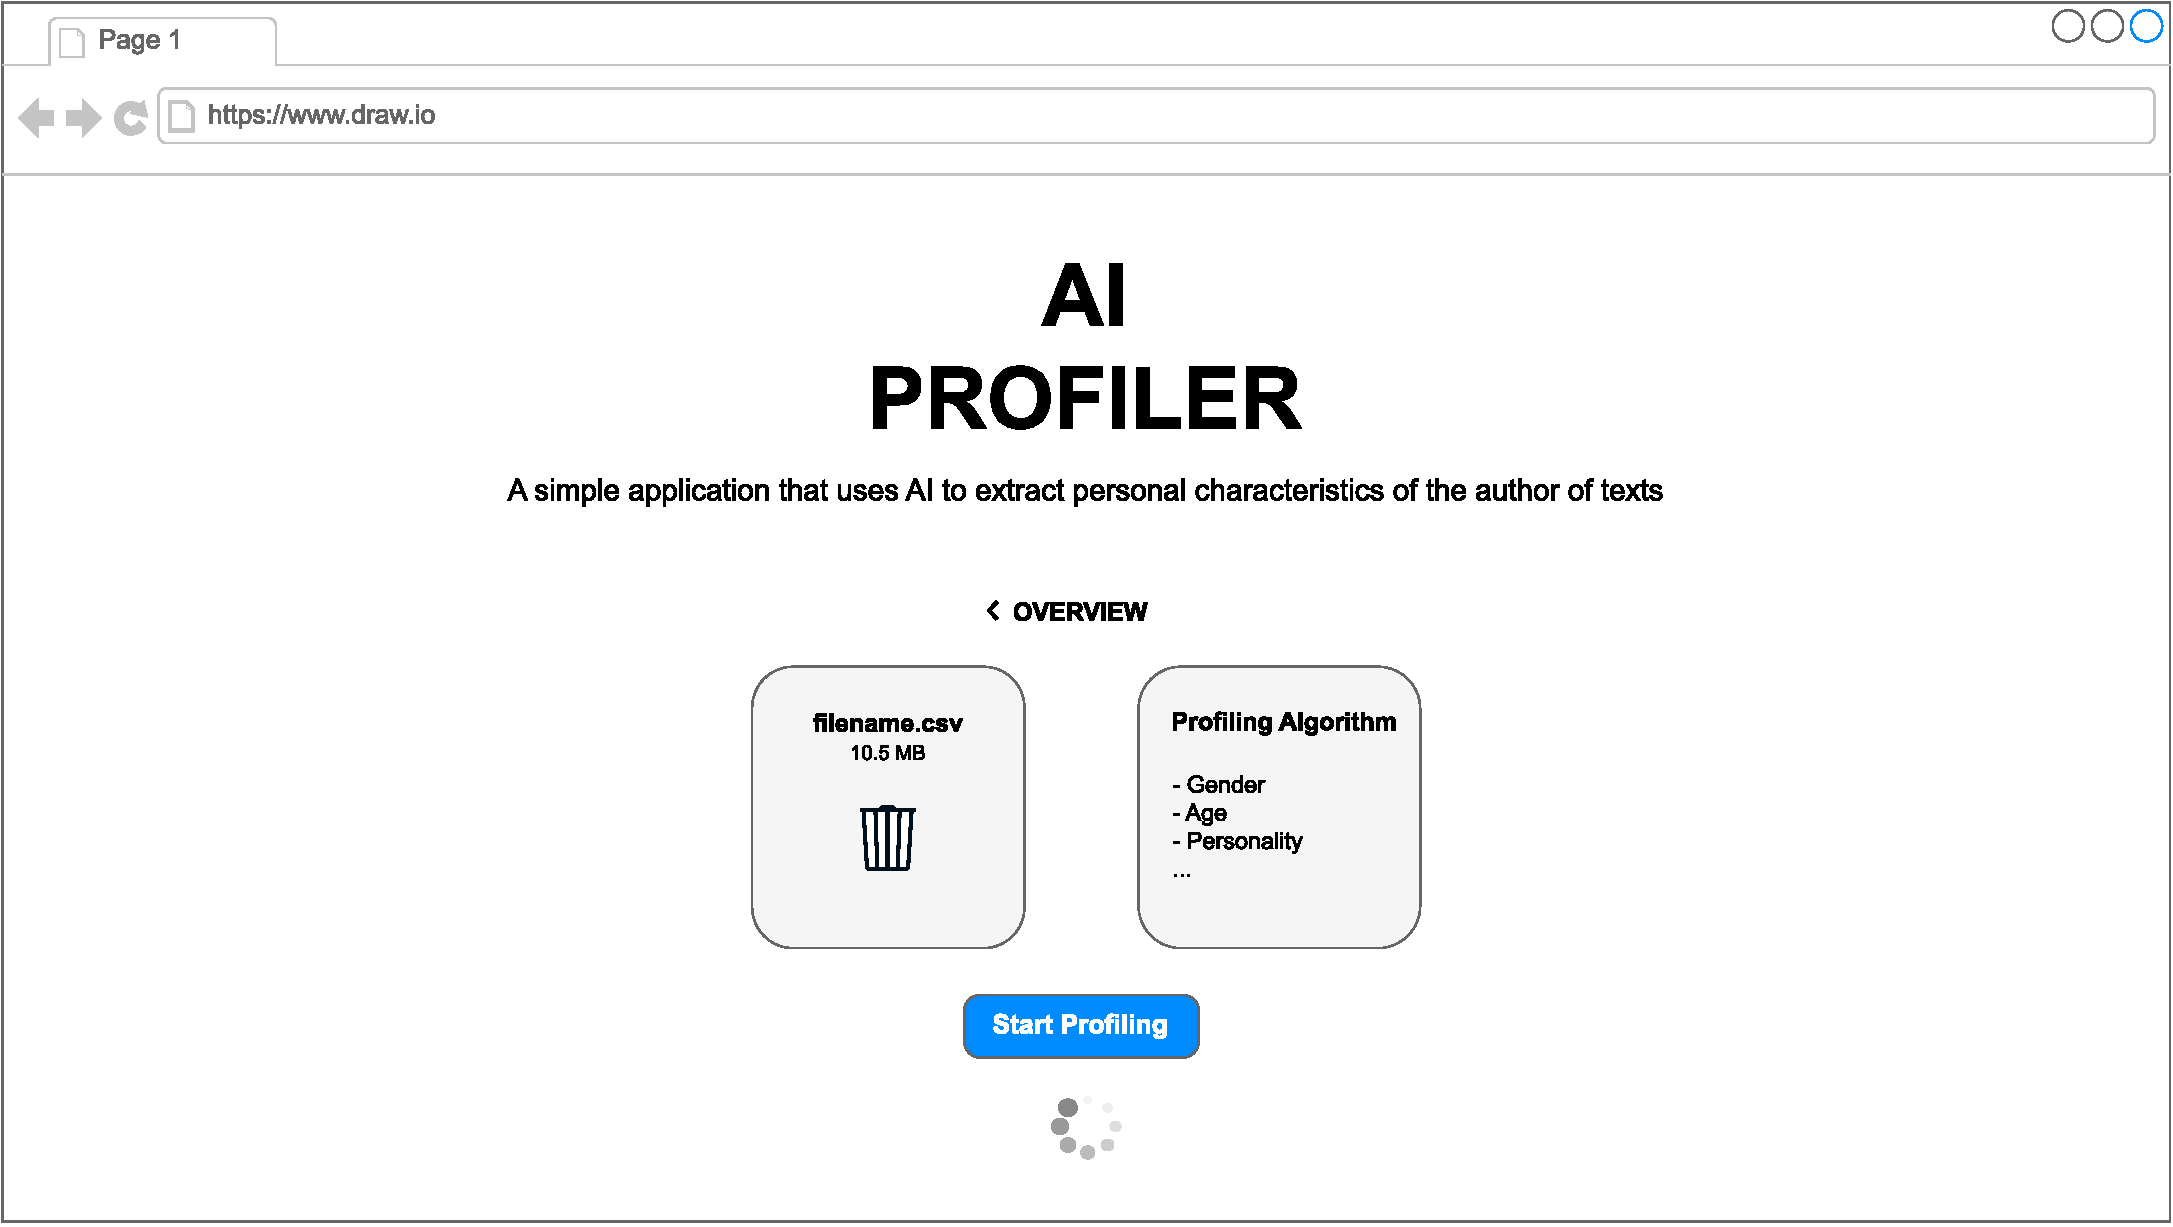
\includegraphics[width=\textwidth]{diagramas/landing-overview.pdf}
	\caption{Prototipo del resumen del perfilado}
	\label{fig:prototipo_resumen_perfilado}
\end{figure}

\bigskip
Con respecto a la pantalla de ejemplos de \textit{datasets}, como se puede ver en la Figura \ref{fig:prototipo_ejemplos_dataset},
se mostrará un pequeño ejemplo de 10-15 líneas aproximadamente. Asimismo, se le dará la opción al usuario de seleccionar el
formato de \textit{dataset}, ya sea NDJSON o CSV, dado que son los que soportará el \textit{backend}.

\bigskip
\begin{figure}[H]
	\centering
	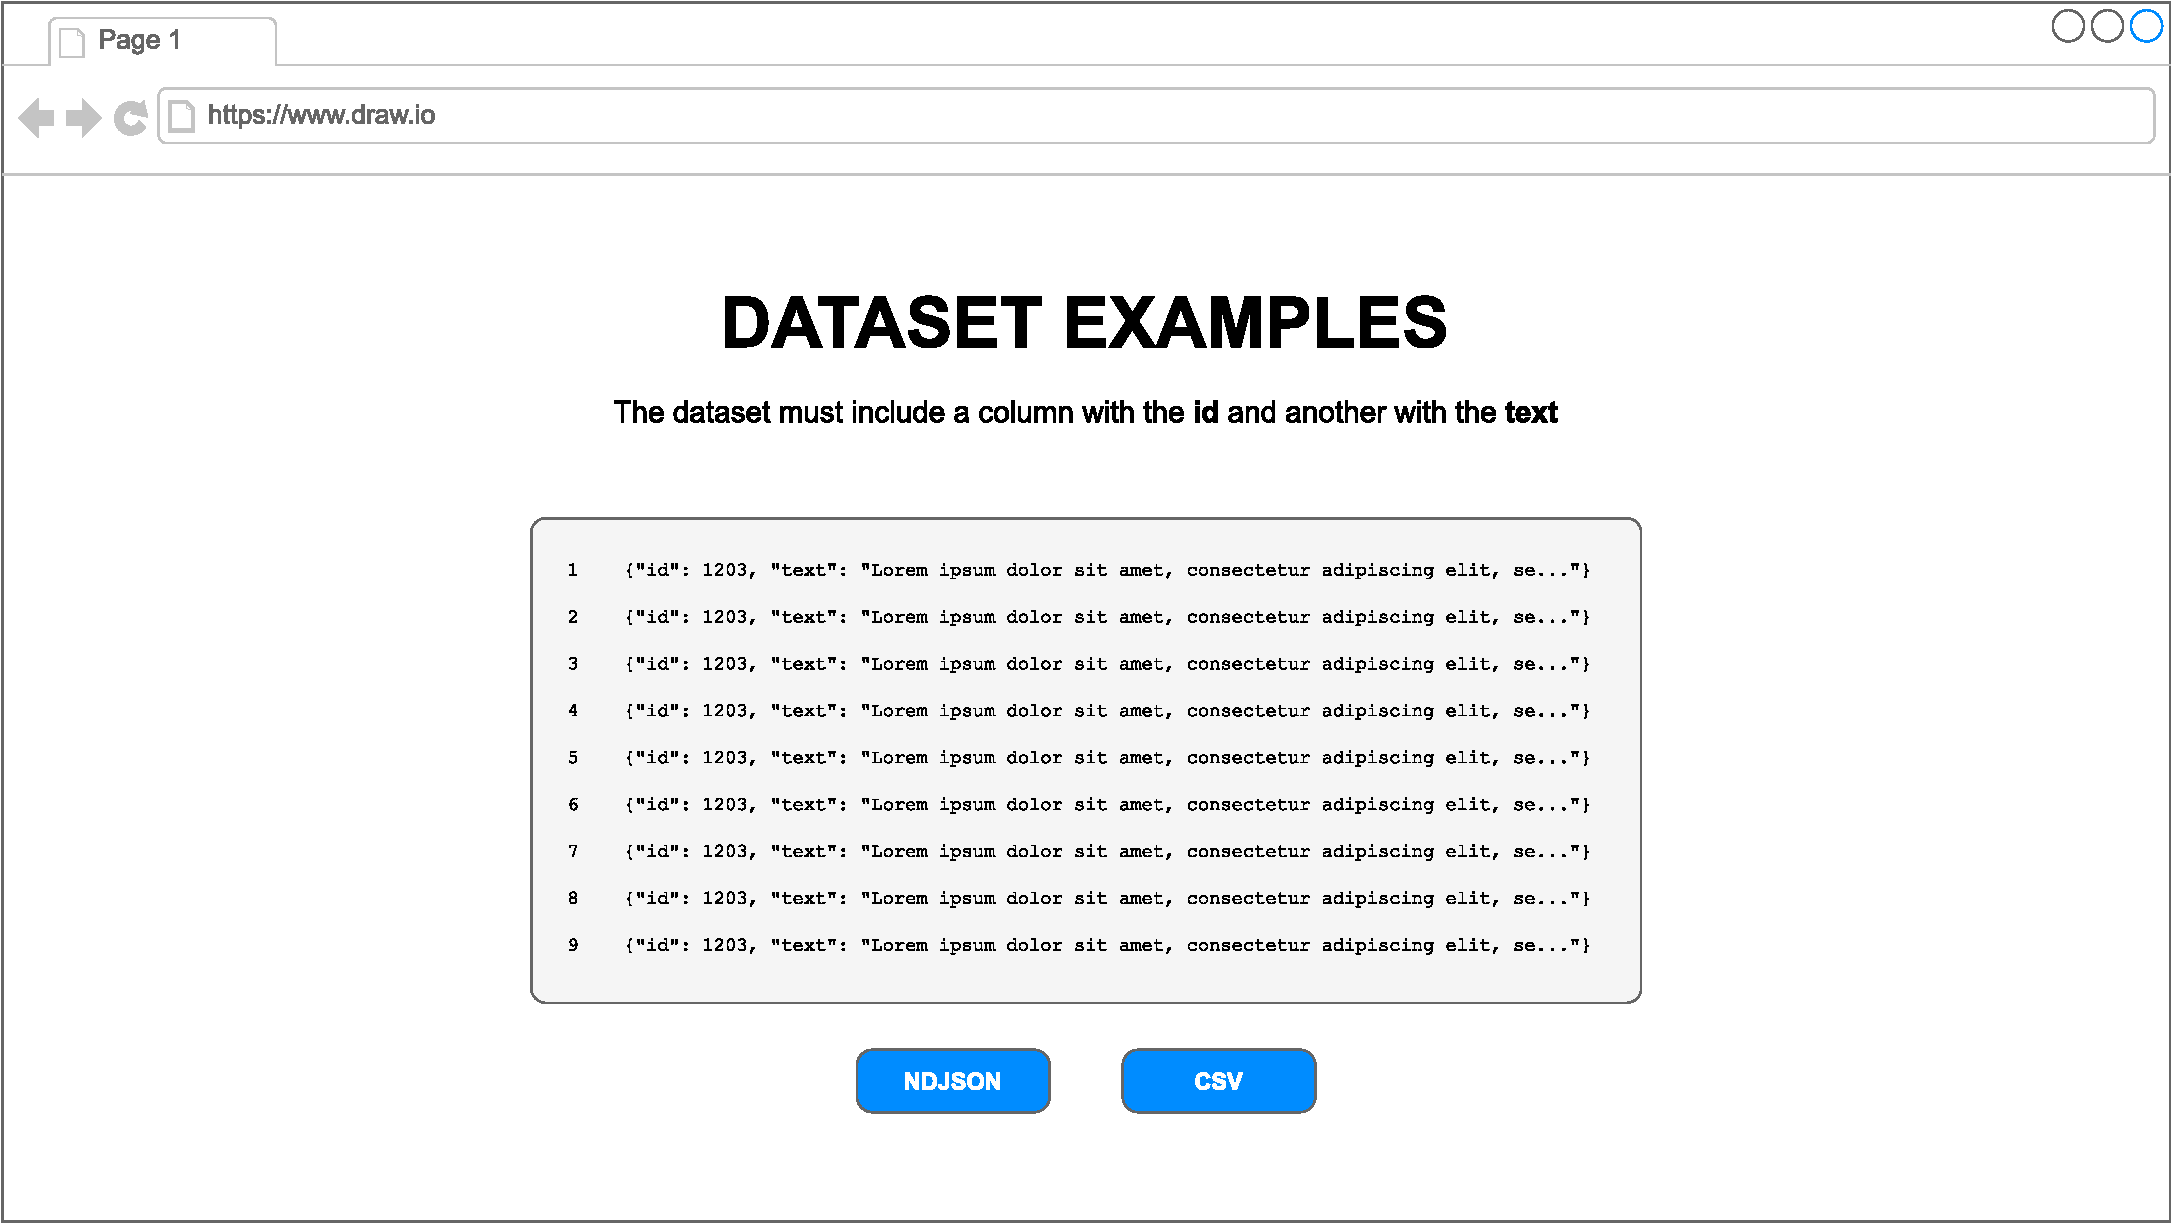
\includegraphics[width=\textwidth]{diagramas/dataset-examples.pdf}
	\caption{Prototipo de la pantalla de ejemplos de dataset}
	\label{fig:prototipo_ejemplos_dataset}
\end{figure}

\bigskip
Cuando el perfilado haya finalizado, se mostrará al usuario un \textit{dashboard} con los resultados obtenidos,
como se puede ver en las Figuras \ref{fig:prototipo_dashboard_martinc} y \ref{fig:prototipo_dashboard_grivas}.
Este \textit{dashboard} contendrá los siguientes gráficos y elementos, los cuales variarán en función del algoritmo utilizado:

\begin{itemize}
	\item \textbf{Datos generales}: El \textit{dashboard} contiene una primera sección en la que aparece información de carácter general
	      como son: el número total de personas perfiladas, el tiempo total del perfilado y el algoritmo utilizado.
	\item \textbf{Lista detallada de personas}: En esta sección se muestra la lista de personas perfiladas de forma paginada, como se establece en la historia de usuario \hyperref[req:hu5]{H5}. Además, la lista
	      permitirá ser ordenada por cada uno de los diferentes campos, según se indica en la historia de usuario \hyperref[req:hu6]{H6}. Para ello, el usuario deberá hacer clic en el nombre de dicho campo, teniendo
	      la opción de, volviendo a clicar, cambiar el sentido de ordenación (ascendente o descendente).
	\item \textbf{Distribución de edad}: Para la distribución de edad, se ha optado por un gráfico de barras sobre otras opciones de representación
	      categóricas como el gráfico circular o el gráfico de anillo. Esto se debe a que, teniendo cinco clases diferentes, el gráfico de barras permite una mejor visualización
	      de los datos y una comparativa más clara entre ellos, dado que es más fácil comparar longitudes que áreas o ángulos. En la parte inferior del gráfico,
	      se mostrará una tarjeta con la edad mediana.
	\item \textbf{Distribución de género}: En cuanto a la distribución de género, en cambio, se ha optado por un gráfico circular, puesto que solo existen dos clases
	      y se desea resaltar la proporción de cada clase con respecto al total. A mayores, se mostrarán debajo del gráfico dos tarjetas con el número de personas
	      de cada género junto con su porcentaje exacto.
	\item \textbf{Distribución de fama \textit{(Martinc)}}: De forma similar a la distribución de género, solo contamos con tres clases diferentes, por lo que
	      se ha elegido un gráfico circular. Resaltar que este gráfico solo se mostrará en el caso de que se haya utilizado el algoritmo de Martinc.
	\item \textbf{Distribución de ocupación \textit{(Martinc)}}: En el caso de la distribución de ocupación, debido a que existen ocho clases distintas, se ha optado
	      por un gráfico de barras. Este gráfico, al igual que el anterior, solo aparecerá si se ha empleado el algoritmo de Martinc para el perfilado.
	\item \textbf{Características personales \textit{(Grivas)}}: Ya que en este caso cada característica personal tendrá asociado un valor decimal entre -0.5 y 0.5,
	      se ha optado por un gráfico de barras. En este sentido, cabe resaltar que para mostrar dicho gráfico, es necesario implementar una funcionalidad que permita
	      seleccionar a una persona de la lista detallada para mostrar sus características personales. Además, este gráfico solo estará disponible si se hace uso del algoritmo de Grivas.
\end{itemize}

\bigskip
\begin{figure}[H]
	\centering
	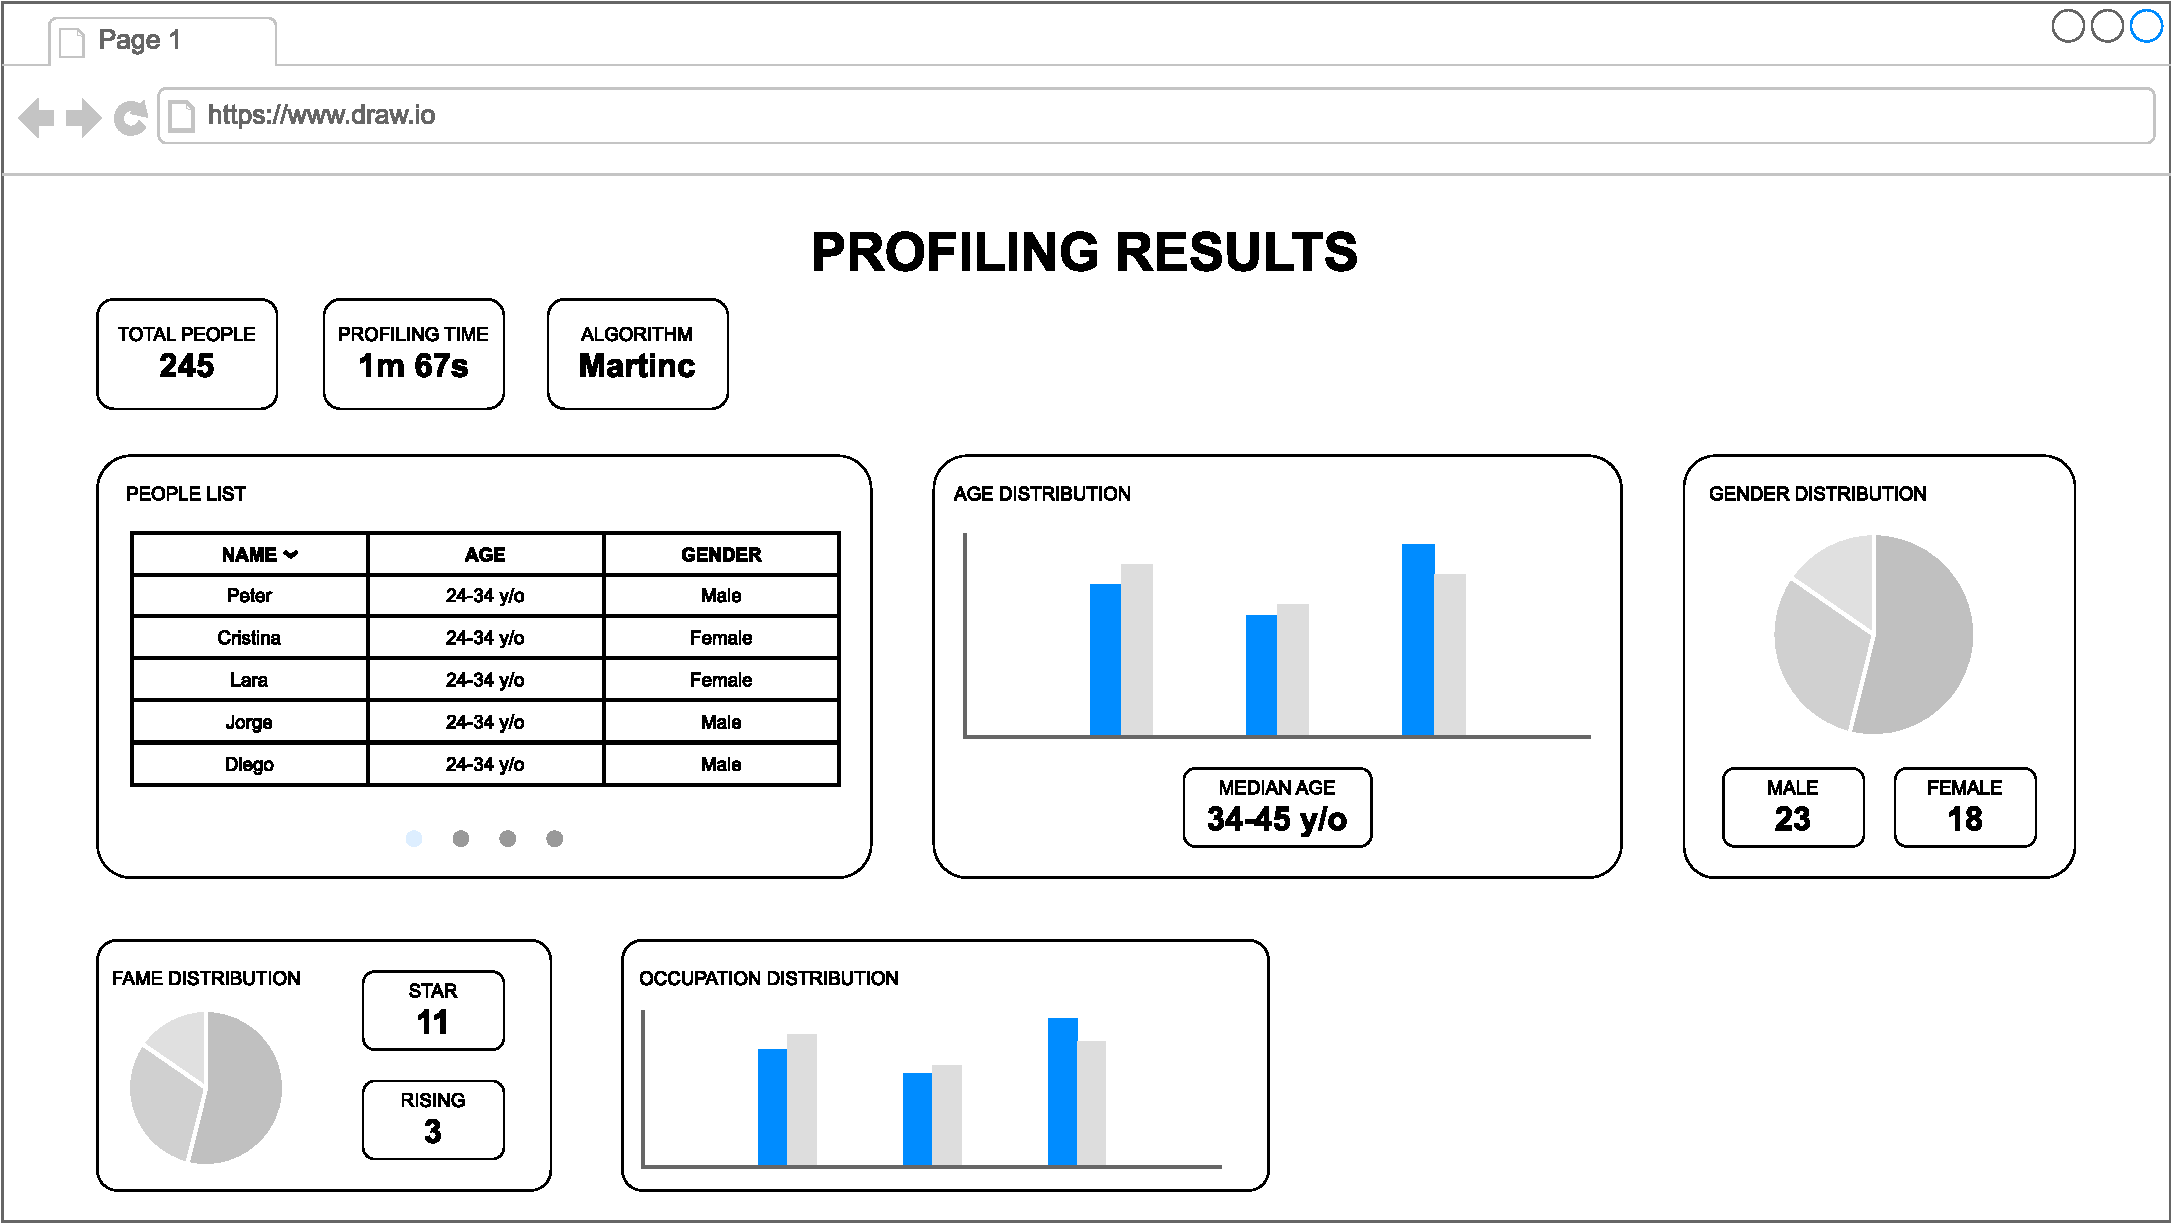
\includegraphics[width=\textwidth]{diagramas/dashboard-martinc.pdf}
	\caption{Prototipo del dashboard utilizando el algoritmo Martinc}
	\label{fig:prototipo_dashboard_martinc}
\end{figure}

\bigskip
\begin{figure}[H]
	\centering
	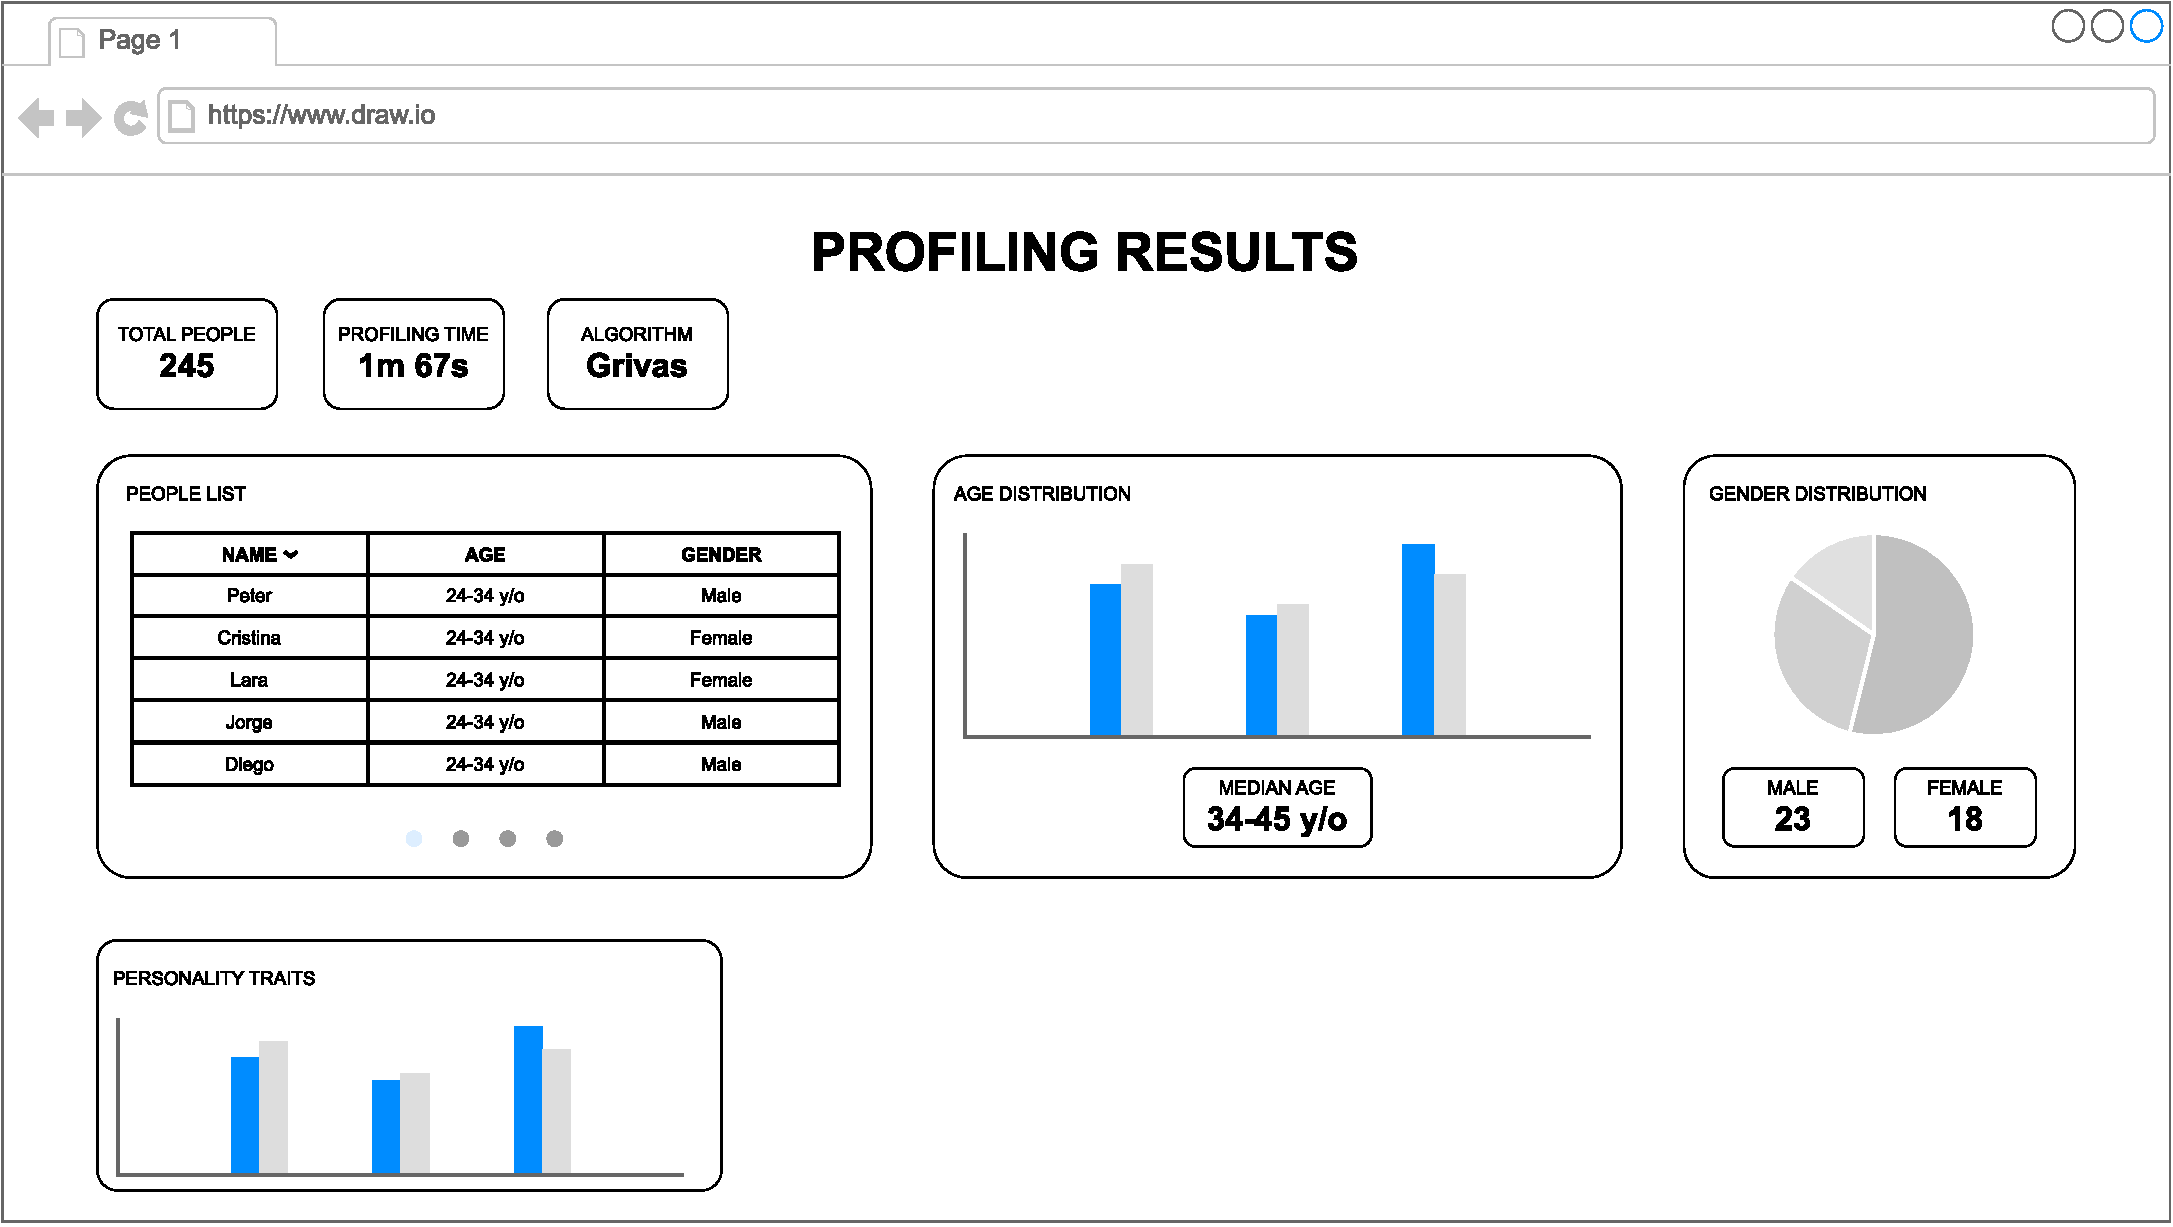
\includegraphics[width=\textwidth]{diagramas/dashboard-grivas.pdf}
	\caption{Prototipo del dashboard utilizando el algoritmo Grivas}
	\label{fig:prototipo_dashboard_grivas}
\end{figure}

\section{\textit{Backend}}

Para analizar la implementación del \textit{backend}, se tomará como referencia el diagrama de clases de la Figura \ref{fig:clases_backend} y se profundizará
en las clases más importantes que lo componen. Asimismo, se estudirá y se justificará cuales han sido los \textit{endpoints} expuestos por el servidor,
representados en la Figura \ref{fig:endpoints}.

\subsection{\textit{Endpoints}}

Dado que el \textit{backend} seguirá una arquitectura REST, se explicarán a continuación los \textit{endpoints} que se han implementado para el servidor, así como los parámetros
que recibe cada uno. Como se puede observar en la Figura \ref{fig:endpoints}, el servidor expone un total de cuatro \textit{endpoints}:

\begin{itemize}
	\item \textbf{/predict}: Como indica la historia de usuario con identificador \textit{1} de la Sección \ref{sec:analisis_requisitos_funcionales}, el usuario
	      debe poder subir su propio dataset de textos para su perfilado. Para ello, se ha implementado este \textit{endpoint} que recibe como parámetros de la URL el
	      nombre del algoritmo de perfilado a utilizar junto al \textit{dataset} utilizado para entrenar el modelo. Además, ya que el método de la petición es POST,
	      será en el cuerpo donde se envíe
	      el archivo con los textos a perfilar. En caso de que el archivo no sea correcto, que el algoritmo no exista o que el \textit{dataset} de entrenamiento
	      no sea válido, se devolverá un error HTTP 400 (\textit{Bad Request}). En caso contrario, se devolverá un identificador correspondiente a la tarea de perfilado
	      que se ha creado de forma asíncrona, generado dinámicamente con la librería uuid \cite{uuidpython} de Python (según el estándar RFC 4122 \cite{rfc4122}) y que coincide
	      con el identificador del documento almacenado en la base de datos.
	      El hecho de no esperar a que el perfilado se complete
	      para devolver una respuesta al usuario evita tener problemas con el tiempo de espera de la petición o \textit{timeout} del \textit{socket} TCP,
	      permitiendo así procesar grandes volúmenes de datos y cumplir con el requisito de escalabilidad \hyperref[req:rnf2]{RNF2}.

	\item \textbf{/train}: Además, ya que el usuario debe poder reentrenar los modelos con los algoritmos disponibles, se ha implementado este \textit{endpoint} de tipo GET.
	      En este caso, se recibe como parámetros de la URL el nombre del algoritmo de perfilado a utilizar junto al \textit{dataset} de entrenamiento. De la misma forma,
	      se validarán los parámetros y, en caso de que sean correctos, se iniciará una tarea asíncrona en el \textit{backend}.

	\item \textbf{/performance}: Puesto que otra de las historias de usuario nos indica que es necesario conocer el rendimiento que tiene los algoritmos,
	      el \textit{backend} expondrá otro \textit{endpoint} de tipo GET que recibe los mismos parámetros que el anterior. La diferencia es que, en este caso,
	      se devolverá un JSON con los valores de rendimiento del algoritmo en lugar de iniciar una tarea asíncrona.

	\item \textbf{/profilings/\{id\}}: Para poder obtener los resultados del perfilado creado de forma asíncrona, este \textit{endpoint} de tipo GET
	      permite recuperarlos de la base da datos haciendo uso del identificador devuelto por la tarea de predicción. En caso de que la tarea
	      no exista, se devolverá un error HTTP 404 (\textit{Not Found}). La respuesta devuelta será un JSON con la estructura mostrada en la Figura \ref{fig:profiling_json}.

	      \begin{figure}[H]
		      \begin{lstlisting}[language=json]
{
	"status": "SUCCESS",
	"algorithm": "martinc",
	"time": 4291,
	"output": [
		{
			"id": "29502",
			"result": {
				"gender": "male",
				"fame": "star",
				"occupation": "sports",
				"age": "35-49"
			}
		},
		{
			"id": "38991",
			"result": {
				"gender": "female",
				"fame": "rising",
				"occupation": "performer",
				"age": "50-XX"
			}
		},
	]
}\end{lstlisting}
		      \caption{Estructura del JSON devuelto por el \textit{endpoint} /profilings/\{id\}}
		      \label{fig:profiling_json}
	      \end{figure}
\end{itemize}

Destacar que, en todos los casos, tanto el algoritmo de Grivas et al. \cite{grivas2015author} como el de Martinc et al. \cite{martinc2019hot}, tienen asociado un \textit{dataset} de entrenamiento por defecto (que coincide
con el utilizado por los autores originales en su publicación), el cual se utilizará en caso de no especificar ninguno en la URL.

\begin{figure}[H]
	\centering
	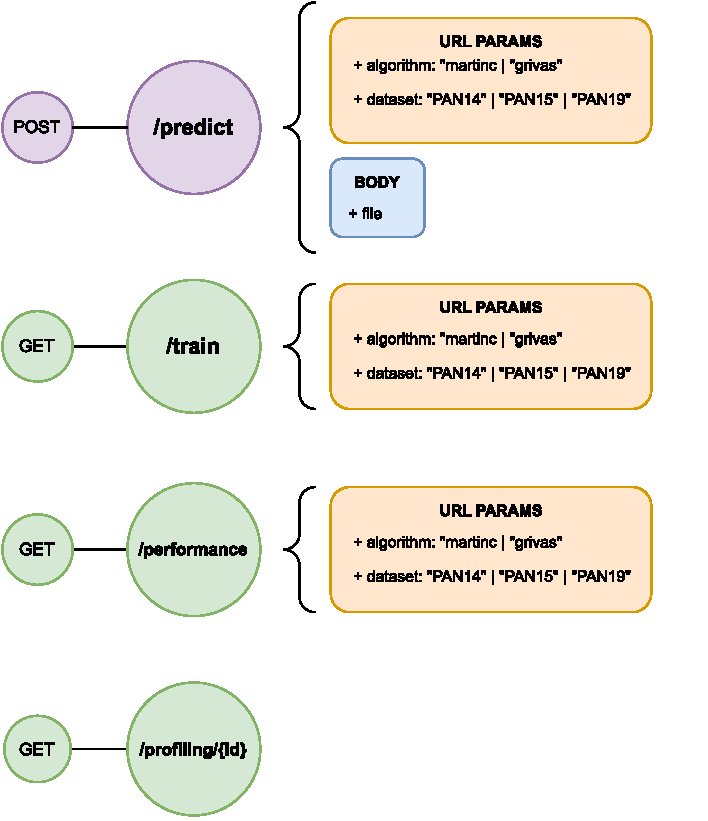
\includegraphics[width=0.5\textwidth]{diagramas/endpoints.pdf}
	\caption{Diagrama de \textit{endpoints} del \textit{backend}}
	\label{fig:endpoints}
\end{figure}

\subsection{Clases}

\bigskip
Como se explicó en la Sección \ref{sec:herramientas_backend}, la estructura del \textit{backend} sigue los principios
del patrón de diseño DDD \cite{ddd}, en el que se distinguen tres capas: la capa de aplicación, la capa de dominio
y la capa de infraestructura.

\bigskip
Nuestro punto de entrada al sistema, es decir, el componente que forma parte de la capa de aplicación, es la clase
\textit{Controller}, el cual se encarga de realizar las siguientes tareas:

\begin{itemize}
	\item Exponer los \textit{endpoints} y recibir los parámetros de entrada, ya sea a través de la URL o del cuerpo de la petición
	      haciendo uso de FastAPI \cite{fastapi}.
	\item Validar dichos parámetros y devolver los errores HTTP correspondientes en caso de que no sean correctos.
	\item Parsear los parámetros de entrada a los tipos de datos que se necesiten.
	\item Realizar la llamada al servicio de la capa de dominio y devolver el valor de retorno encapsulado en una respuesta HTTP.
\end{itemize}

\bigskip
En la capa de dominio, una vez los datos han sido validados y parseados, el \textit{ProfilingService} es el encargado de orquestar
las diferentes llamadas y delegar la lógica de negocio a las distintas entidades.

\bigskip
La más importante de ellas es la clase \textit{ProfilingAlgorithm},
una clase abstracta que define la interfaz que deben implementar todos los algoritmos de perfilado incluyendo las tres funciones principales:
\textit{predict()}, \textit{train()} y \textit{get\_performance()}. En este sentido, es importante mencionar que los algoritmos elegidos no estaban implementados
pensando en formar parte de una aplicación más grande, por lo que fue necesario realizar una adaptación manual para cumplir con la interfaz de
la clase heredada, explicada en profundiad en la Sección \ref{sec:adaptacion_algoritmos}.

\bigskip
Otra entidad importante de la capa de dominio es la clase \textit{PredictDataset}, que representa el \textit{dataset} que proporciona el usuario
para realizar la predicción. Dado que los algoritmos de perfilado requieren que el \textit{dataset} tenga un formato específico (en este caso
ambos solo procesan NDJSON), es necesario implementar conversores que transformen el archivo de entrada a dicho formato por lo que
fue necesario crear las clases \textit{CsvToNdjsonConverter} y \textit{NdjsonToCsvConverter}.

\bigskip
También existe una clase llamada \textit{TrainDataset}, que representa
el \textit{dataset} que se utiliza para entrenar y validar el modelo. Esta clase abstracta contiene la locacalización de los elementos
del conjunto de entrenamiento y test, así como también un nombre que la identifica. Esto nos permite la incorporación de nuevos \textit{datasets} creando simplemente
una nueva clase que herede de \textit{TrainDataset}, posibilitando la generación de modelos haciendo uso de diferentes conjuntos de entrenamiento de forma sencilla y automática.

\bigskip
Finalmente, en la capa de dominio, se encuentra la clase abstracta \textit{ProfilingRepository}, la cual define la interfaz que deben implementar
los repositorios de tecnologías de bases de datos concretas, ya sean relacionales, no relacionales o de otro tipo.

\bigskip
Ya en la capa de infraestructura, es decir, donde se almacenan todos los componentes externos con los que interactúa el dominio, se encuentran las clases que implementan
la interfaz definida por el \textit{ProfilingRepository}. En nuestro caso, ya que se decidió optar por MongoDB como base de datos, solo existe
la clase \textit{MongoProfilingRepository}, la cual se encarga de realizar las operaciones CRUD (del inglés \textit{Create, Read, Update, Delete}) sobre la base de datos, así
como de establecer y mantener las conexiones con la misma.

\bigskip
\begin{figure}[H]
	\centering
	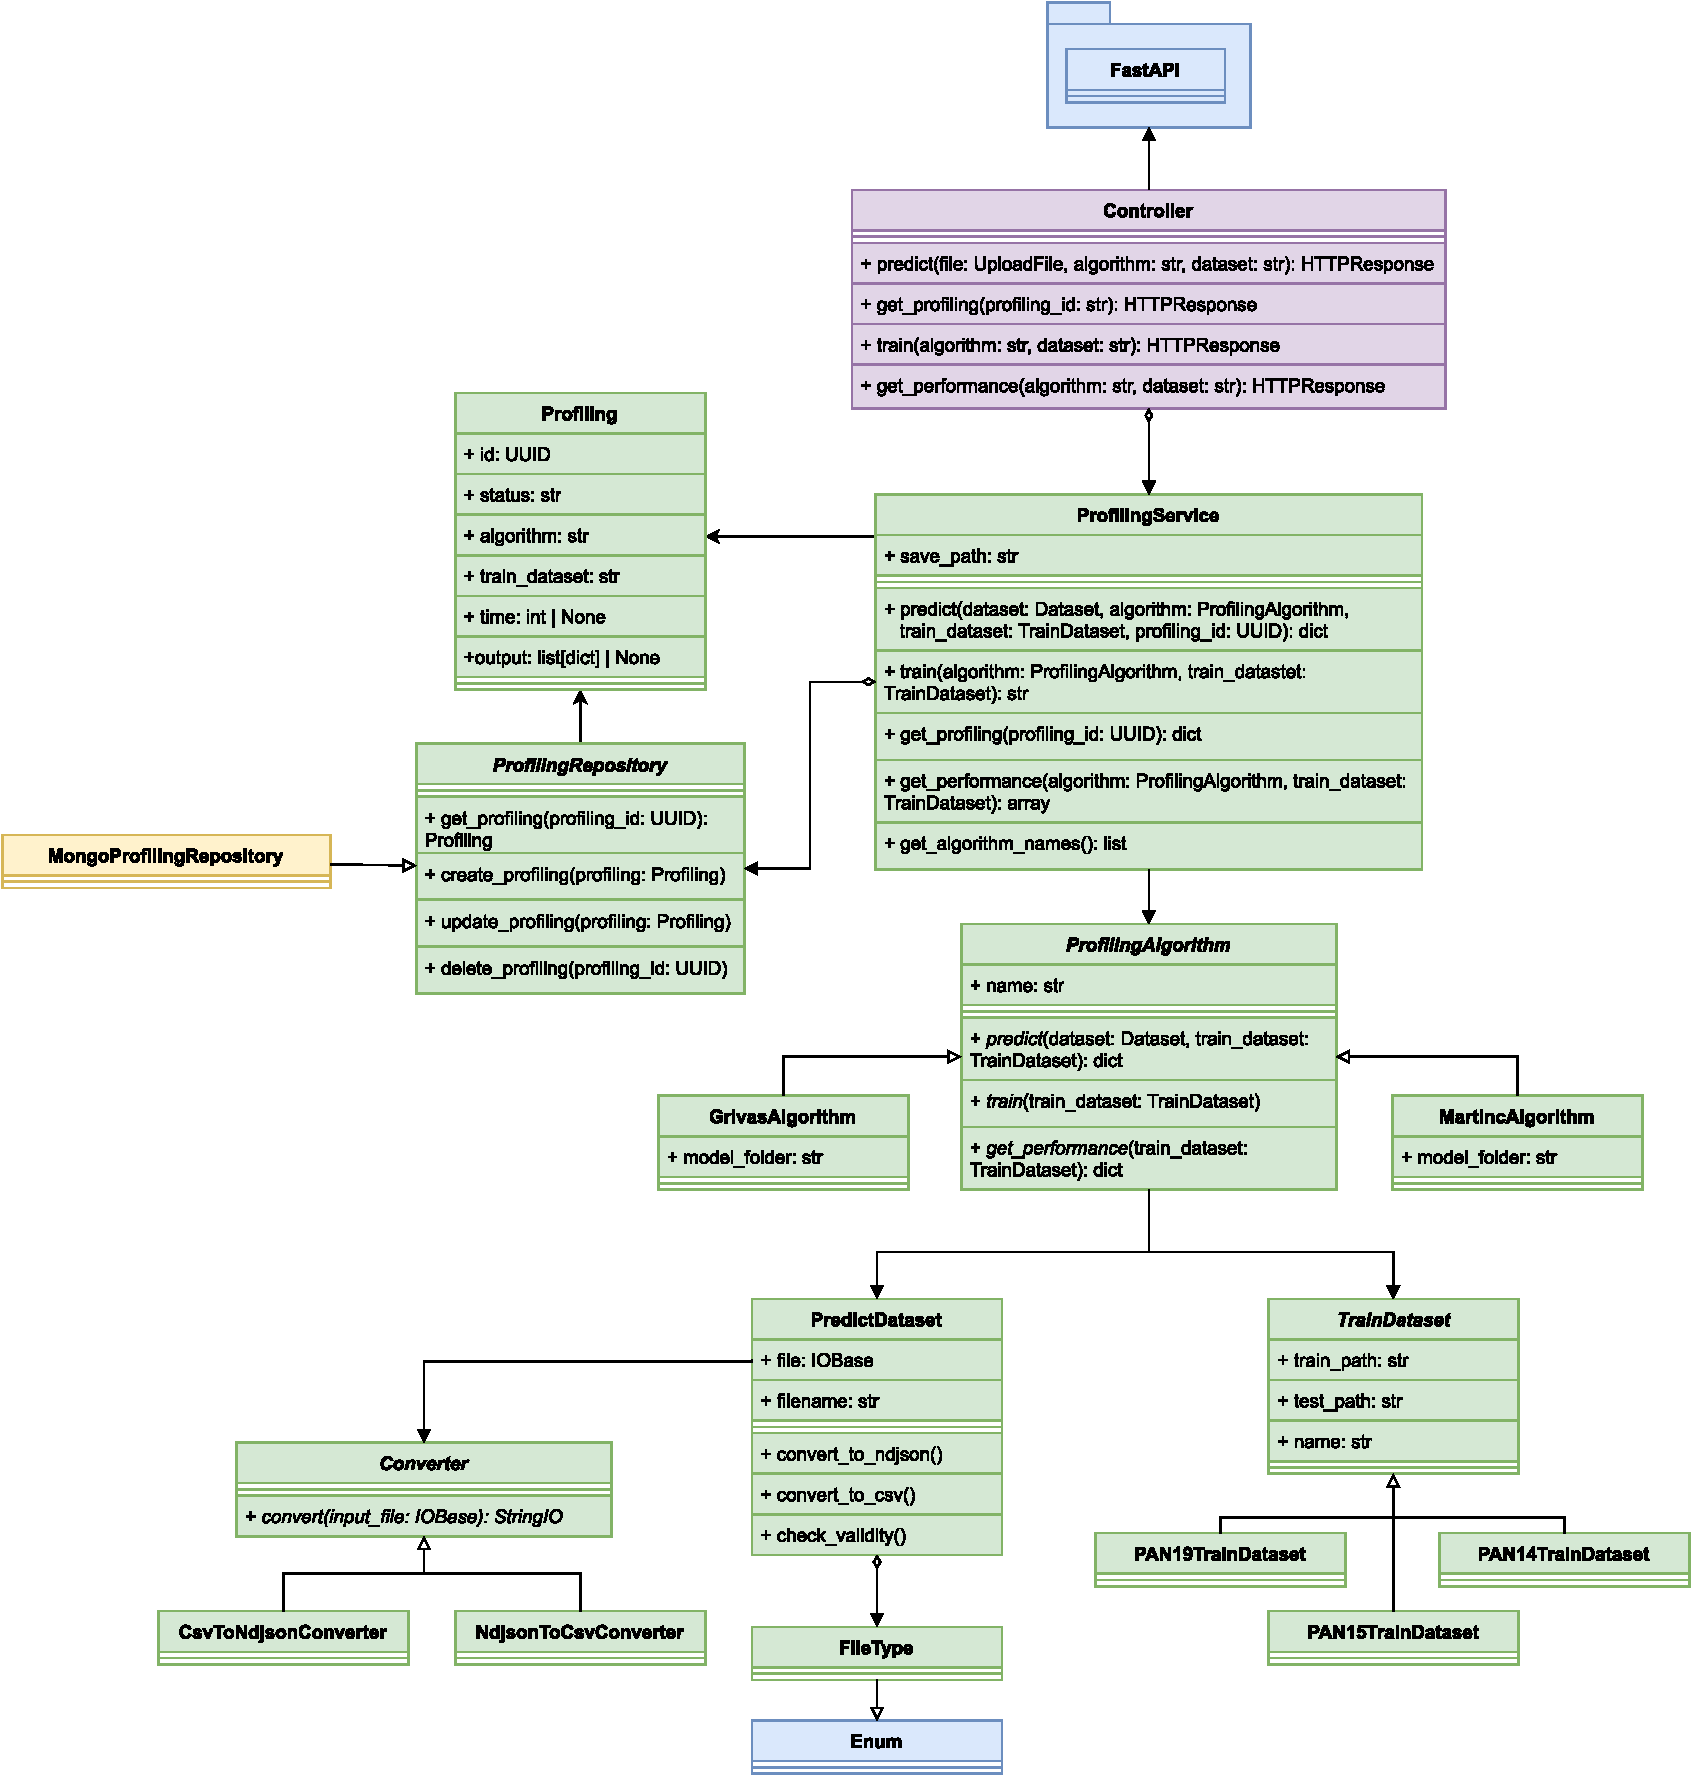
\includegraphics[width=\textwidth]{diagramas/clases_back.pdf}
	\caption{Diagrama de clases de la implementación del \textit{backend}}
	\label{fig:clases_backend}
\end{figure}

\section{\textit{Frontend}}

En lo que respecta a la implementación del \textit{frontend}, como se explicó en la Sección \ref{sec:herramientas_frontend}, se optó
por utilizar NextJS como \textit{framework} de desarrollo, el cual está basado en React. Así, teniendo esto en cuenta y apoyándonos
en el diagrama de clases de la Figura \ref{fig:clases_frontend}, analizaremos
las clases más relevantes del proyecto y su relación con el resto de módulos y componentes.

\bigskip
Primero, como elemento principal que conforma la interfaz de usuario, estarían todas las páginas que se encuentran en el módulo \textit{pages}, es decir,
la página principal (\textit{Home}) y la página de resultados (\textit{Results}).

\bigskip
Como se ve reflejado en el diagrama, cada página está formada por varios componentes, los cuales se almacenan dentro del módulo \textit{components}.
En este sentido, el componente \textit{Chart} es uno de los más complejos e interesantes, dado que en él reside toda la lógica y la configuración común
de los gráficos que se muestran en el \textit{dashboard} de la página de resultados. Otros componentes importantes son el \textit{UploadDataset},
el cual se encarga de gestionar los eventos de \textit{drag and drop} y de la subida de archivos; el componente \textit{AlgorithmCard}, que
presenta la información de las caraterísiticas que perfila cada algoritmo y se ocupa de mostrar el \textit{tooltip} con la información detallada;
o el componente \textit{PeopleList}, el cual se hace cargo de manejar la paginación, la ordenación y la selección de la lista de personas.

\bigskip
Es importante
destacar aquí el hecho de que cada uno de los componentes tiene una hoja de estilos propia gracias a la utilización de los módulos CSS \cite{cssmodules}. A su vez
se buscó sacarle partido a SASS, haciendo uso de variables globales que definen colores o distancias; empleando el anidamiento para una mejor
estructuración de los estilos; y utilizando los \textit{mixins}, esto es, funciones que permiten reutilizar código CSS para, por ejemplo, simplificar la implementación de las \textit{media queries}. En este
sentido, para cumplir con el requisito no funcional de portabilidad \hyperref[req:rnf3]{RNF3},
era necesario que la aplicación fuese \textit{responsive}, es decir, adaptable a cualquier tamaño de pantalla, desde móviles a monitores.

\bigskip
Por otro lado, ya que algunos componentes y páginas necesitan realizar peticiones al \textit{backend}, es necesario implementar un servicio
que contenga la lógica de la comunicación y exponga funciones que faciliten su uso. De esta tarea se encarga la clase abstracta \textit{ProfilingService},
la cual define funciones estáticas tales como \textit{getProfiling()} o \textit{predict()} que abstraen al resto de componentes de la lógica de las peticiones HTTP.
Dicho servicio hace uso por debajo de \textit{fetch}, una API nativa de JavaScript muy flexible que permite programar casi cualquier funcionalidad
relacionada con peticiones HTTP. Asimismo, ya que la asincronía es un concepto muy extendido y necesario en el desarrollo web, se optó
por usar las \textit{Promises} de JavaScript, las cuales permiten realizar operaciones asíncronas de forma muy sencilla.

\bigskip
Por último, como toda aplicación tipada, es necesario definir un modelo de datos que represente cada entidad. En este sentido, se ha optado
por el uso de enumeraciones o \textit{enums} para representar la mayor parte de los datos, tales como los algoritmos de perfilado, los géneros,
las edades o los rasgos personales. Asimismo, se ha creado una clase \textit{Person} que aúna todas las características
perfiladas de una persona junto a su nombre. Finalmente, para representar los datos enviados por el \textit{backend}, se ha definido la clase \textit{ProfilingDto},
la cual, en última instancia, permite realizar la conversión a la clase \textit{Profiling} empleada por el resto de la aplicación.

\bigskip
\begin{figure}[H]
	\centering
	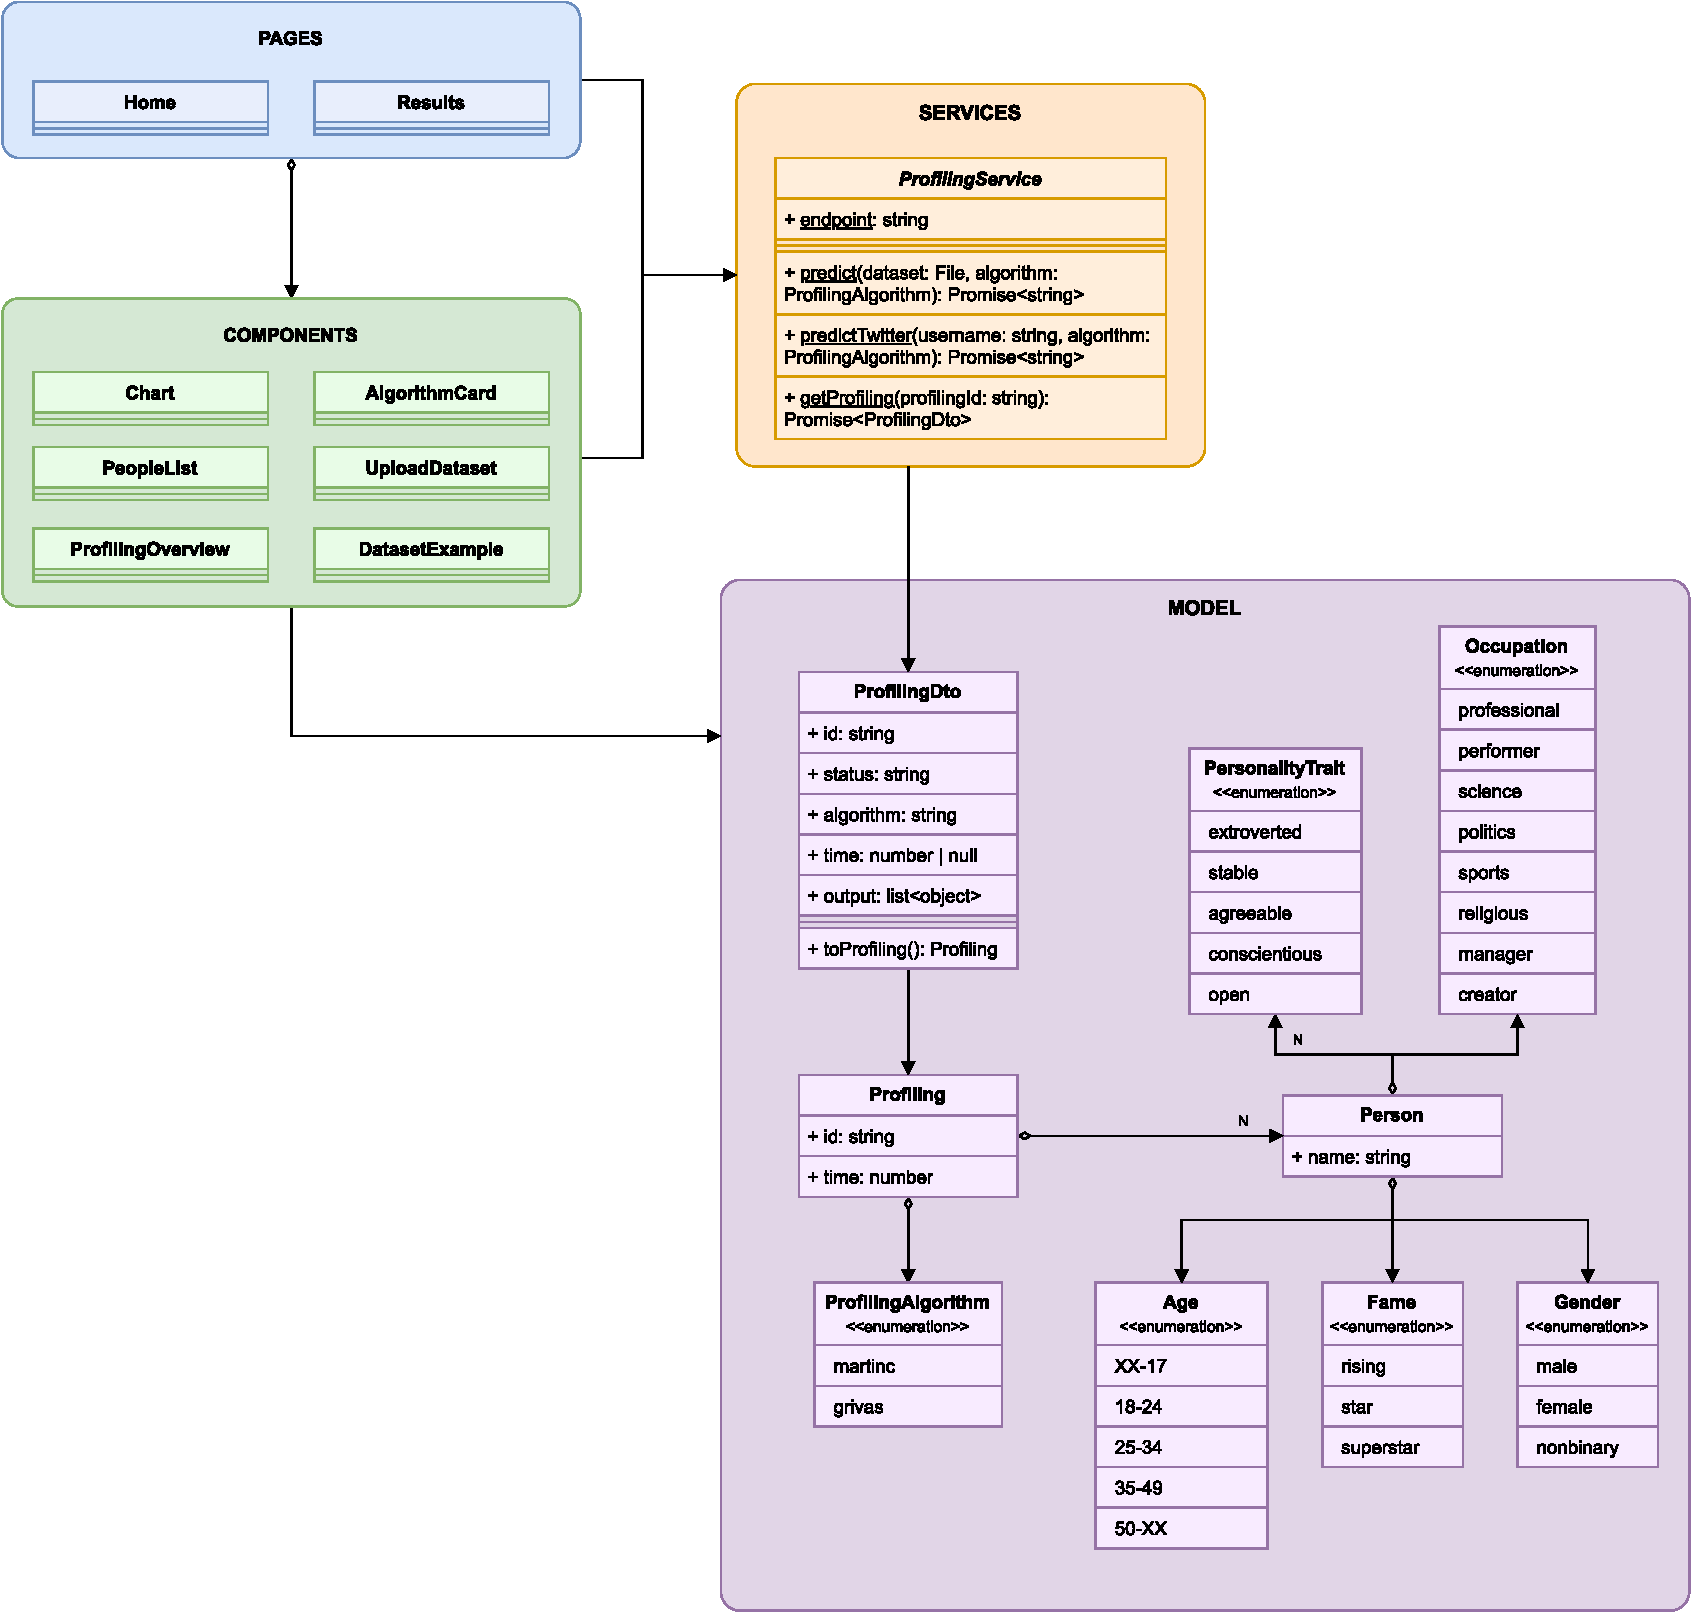
\includegraphics[width=\textwidth]{diagramas/clases_front.pdf}
	\caption{Diagrama de clases de la implementación del \textit{frontend}}
	\label{fig:clases_frontend}
\end{figure}
